\documentclass[12pt, a4paper, titlepage]{report}
\usepackage[a4paper,top=2.5cm,bottom=2cm,left=2cm,right=2cm]{geometry}
\usepackage[italian]{babel}
\usepackage[hidelinks]{hyperref}
\usepackage{graphicx}
\usepackage{algorithm}
\usepackage{capt-of}
\usepackage{amsmath}
\usepackage{longtable}
\usepackage{caption}
\usepackage{booktabs}
\usepackage{algpseudocode}
\usepackage{makecell}
\usepackage[utf8]{inputenc}
\usepackage{fixltx2e}
\usepackage{listings}
\usepackage{hyperref}
\usepackage{makecell}
\usepackage{changepage}
\usepackage{paracol}
\usepackage{siunitx}
\usepackage{lipsum}
\usepackage{float}
\usepackage{subfig}

\usepackage[swapnames]{frontespizio}

\usepackage{fancyhdr}
\usepackage{lastpage}
%\pagestyle{fancy}
%\fancyhf{}
%\cfoot{Pagina \thepage\ di \pageref{LastPage}}

\setcounter{tocdepth}{6}
\setcounter{secnumdepth}{6}
\newcommand\tab[1][1cm]{\hspace*{#1}}
\renewcommand{\thesection}{\arabic{section}}%
\newcommand{\myparagraph}[1]{\paragraph{#1}\mbox{} \mbox{}}
\newcommand{\tommaso}{Tommaso Carraro}
\newcommand{\alberto}{Alberto Bezzon}
	
\begin{document}
	
	\begin{frontespizio}
		\begin{Preambolo*}
			\usepackage{fourier}
		\end{Preambolo*}
		\Universita{Padova}
		\Dipartimento{Matematica}
		\Scuola{Corso di Mobile Programming and Multimedia}
		\Filigrana [height=7.5cm,before=0.28,after=1]{logo-unipd.png}
		\Titolo{\vspace{8cm}\Huge{Relazione del progetto SmartOrder}}
		\Relatore{Alberto Bezzon 1211016\\Tommaso Carraro }
		\NRelatore{Studenti}{}
		\Annoaccademico{2018-2019}
	\end{frontespizio}
	
	%\maketitle
	%\pagestyle{empty}
	\setcounter{page}{2}
	\tableofcontents
	\newpage
	\listoffigures
	\newpage
	\listoftables
	\setcounter{table}{0}
	\newpage	    
	\renewcommand*{\arraystretch}{2}
	\pagestyle{fancy}
	\fancyhf{}
	\rhead{Relazione del progetto SmartOrder}
	\lhead{Corso di Mobile Programming and Multimedia \\ Università di Padova}
	\cfoot{\thepage}
	%\setlength{\headsep}{2cm}
	
	\section{Introduzione}
	Il progetto consiste nello sviluppo di un'applicazione, chiamata SmartOrder, per effettuare ordini dal proprio fornitore. L'applicazione è stata sviluppata per smartphone utilizzando il framework cross-platform PhoneGap.
	
	\section{Il framework cross-platform adottato}
	Il framework cross-platform scelto per lo sviluppo dell'applicazione è PhoneGap. La scelta è ricaduta su questo framework perché un'applicazione sviluppata con PhoneGap è un'applicazione web a cui si aggiunge il motore di rendering webkit. Inoltre, per un'applicazione semplice come SmartOrder permette di ottenere delle buone performance.
	Poiché è un'applicazione web, i linguaggi sono HTML, CSS e Javascript. Questi linguaggi sono a noi noti e questo ci ha permesso di sviluppare un'applicazione evitando di imparare un nuovo linguaggio.
	
	\section{Tutorial}
	Le pagine realizzate sono le seguenti:
	\begin{itemize}
		\item login.html;
		\item homepage.html;
		\item order.html;
		\item article.html;
		\item articles.html;
		\item newpage.html;
		\item inventory.html;
	\end{itemize}
	Ad ognuna di queste pagine è associato un foglio di stile e un file Javascript; inoltre sono presenti un file CSS e un file Javascript generali.
	
	\subsection{Informazioni utili all'utilizzo}
	Per poter utilizzare l'applicazione è necessario essere connessi ad Internet, in quanto l'applicazione scarica i dati da un server. Abbiamo notato che con la rete Eduroam e Studenti.math.unipd.it dell'università, l'applicazione non funziona. Inoltre la mail deve essere certificata da Amazon 
	
	\section{Mobile design}
	In questa sezione vengono descritte tutte le scelte effettuate ai fini di una corretta progettazione dell'applicazione. Seguono varie sottosezioni, una per ogni elemento dell'app, in cui vengono spiegati gli elementi e le motivazioni relative alla loro progettazione.
	
	\subsection{Bottoni}
	Nelle pagine Carrello, Modifica o Aggiungi sono presenti dei bottoni nella parte bassa dello schermo. L'applicazione richiede una frequente modifica dei dati quindi i controlli sono stati posizionati in una zona semplice da raggiungere e seguendo la regola "Content always on top" si è preferito inserire questi bottoni in basso, infrangendo così la regola pratica che in Android i controlli devono essere posizionati nella parte alta dello schermo. Questi bottoni sono più grandi rispetto a quelli situati nella parte centrale in quanto si è rispettata l'immagine in Figura \ref{fig:dimvspos}.
	\begin{figure}[H] 
		\centering
		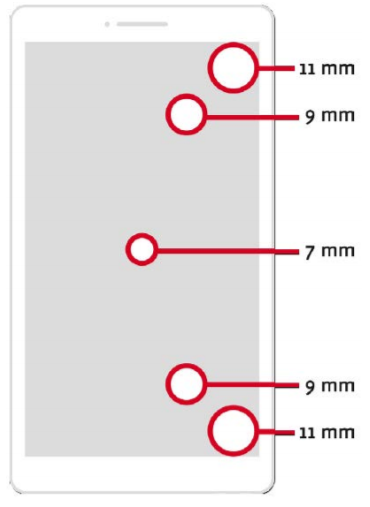
\includegraphics[width=0.3\textwidth]{img/dimvspos}
		\caption{Dimensione vs. posizione dei bottoni}
		\label{fig:dimvspos}
	\end{figure}
	\noindent I bottoni al centro sono più piccoli ma sono comunque sufficientemente distanti da evitare il tap su un altro bottone.
	
	\subsection{Menu}
	\begin{figure}[H] 
		\centering
		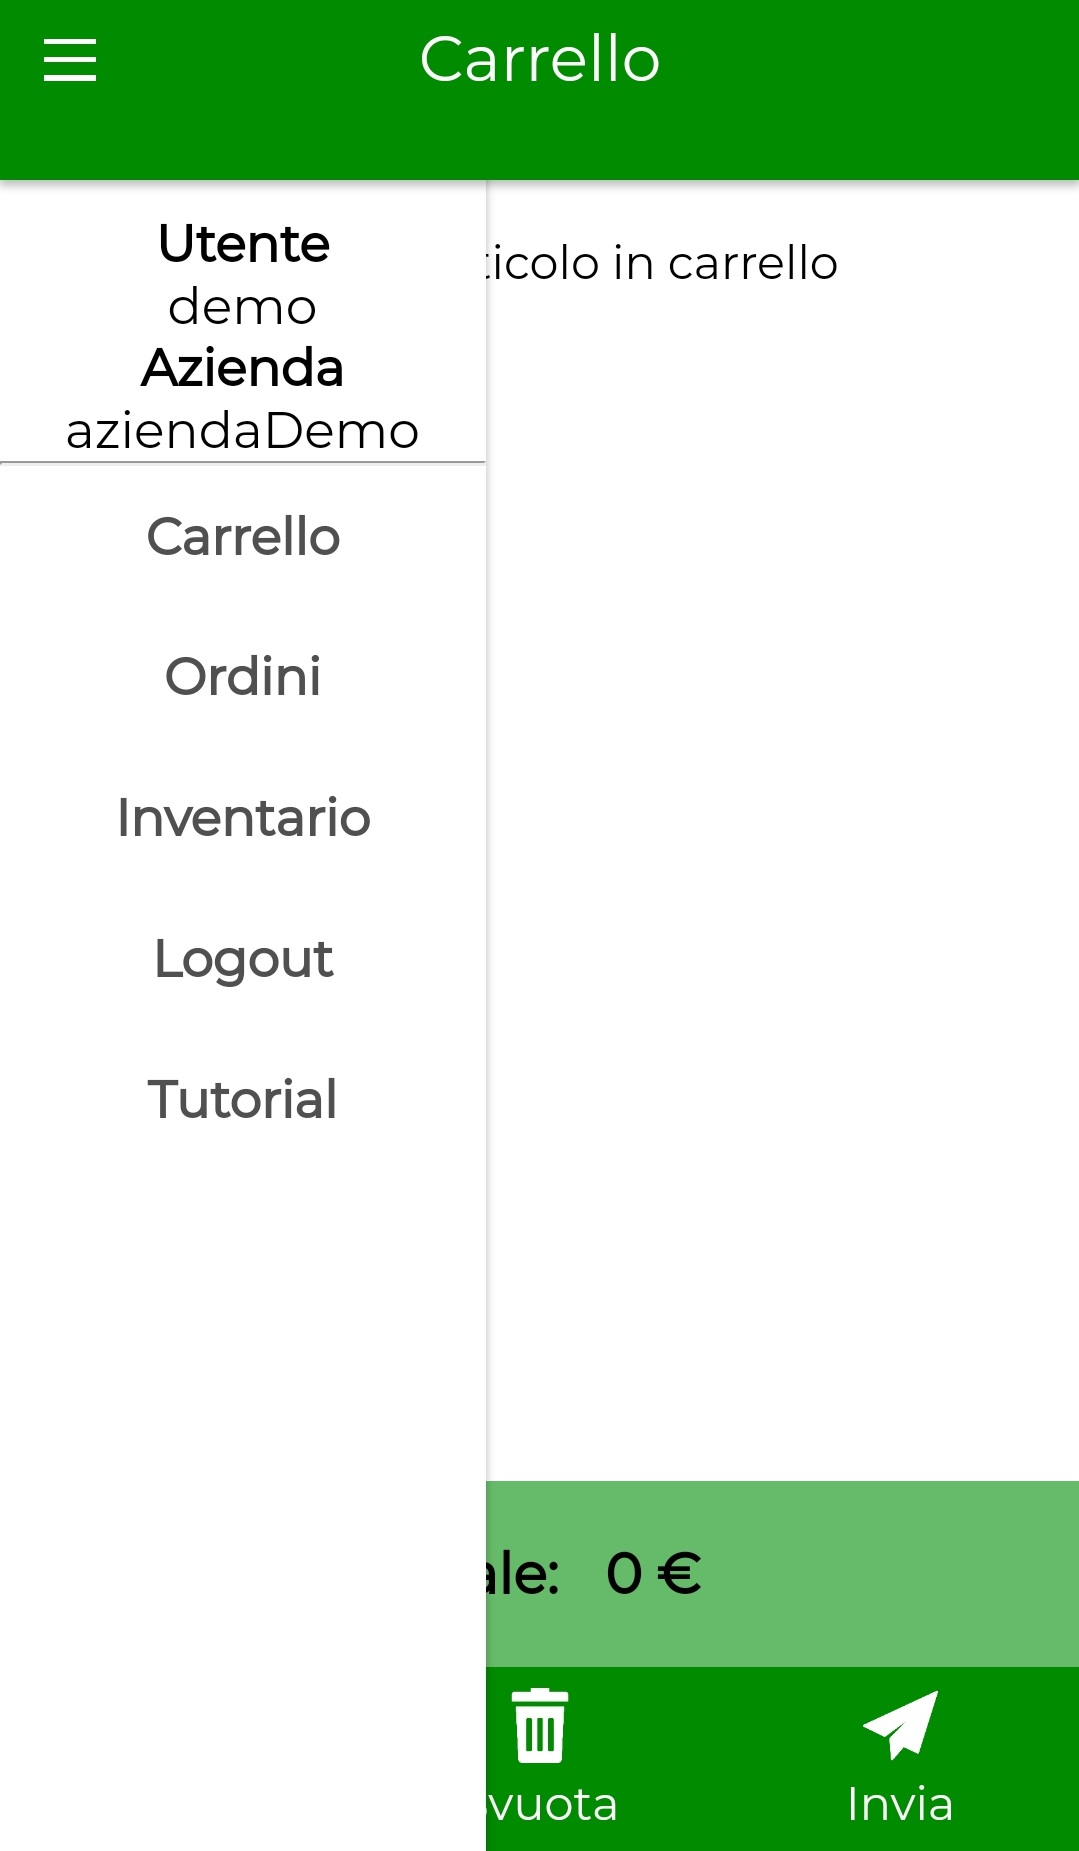
\includegraphics[width=0.3\textwidth]{img/menu}
		\caption{Menu dell'applicazione}
		\label{fig:menu}
	\end{figure}
	Il menu dell'applicazione è rappresentato in Figura \ref{fig:menu}. Per aprire il menu è presente il classico bottone del menu "hamburger" sulla barra in alto a sinistra. Il menu è suddiviso in due parti: 
	\begin{itemize}
		\item Informazioni relative all'utente che ha effettuato il login nell'applicazione, in particolare vengono visualizzati il nome dell'utente e il nome dell'azienda. Queste due informazioni non sono modificabili e pertanto sono nella parte alta del menu dato che non è possibile interagire con esse;
		\item L'insieme di link che permettono di navigare tra le pagine dell'applicazione, in particolare sono disponibili i link al carrello, alla lista degli ordini, all'inventario. Inoltre, è disponibile un bottone "Logout" che permette di effettuare il logout dall'applicazione. Premendo su ognuno di questi viene cambiata l'interfaccia, pertanto essendo possibile interagire con essi, sono stati posizionati nella confort zone.
	\end{itemize}

	\subsection{Pagina ordini}
	In generale, è una buona regola non affollare le interfacce. In particolare nella pagina ordini le informazioni sui vari ordini sono disponibili facilmente, mentre i dettagli di ogni ordine sono rimandati ad un'interazione successiva (progressive disclosure). Questo approccio favorisce la chiarezza sulla quantità di informazioni fornite ed evita l'affollamento dell'interfaccia.
	
	\subsection{Tastiera}
	L'utilizzo della tastiera è necessario in tre casi:
	\begin{itemize}
		\item Per inserire le credenziali necessarie per il login all'applicazione;
		\item Per effettuare la ricerca di un articolo;
		\item Per inserire la quantità del prodotto che si vuole inserire nel carrello.
	\end{itemize}
	Nel caso della quantità sono stati messi a disposizione due pulsanti (+/-) che, rispettivamente, aumentano e diminuiscono la quantità. Inoltre, se si desidera inserire un valore, premendo sulla textbox compare una tastiera con soli numeri in modo da aumentare la velocità dell'utente a digitare.
	
	\subsection{Tutorial}
	La prima volta che l'utente accede all'applicazione, dopo aver effettuato il login, viene visualizzato il tutorial per utilizzare l'applicazione. Il tutorial fornisce le istruzioni più importanti per l'utilizzo dell'applicazione, in quanto l'applicazione è abbastanza intuitiva. Alla fine del tutorial è presente un bottone che permette di iniziare ad utilizzare l'applicazione. Il tutorial comunque sarà disponibile dal menu, nel caso l'utente non ricordasse come utilizzare l'app.
	
	\subsection{Elementi nativi}
	Gli elementi nativi dell'applicazione sono la fotocamera e i dialog.
	
	Riteniamo che l'applicazione soddisfi i primi tre livelli della piramide di Maslow rimappata sui bisogni degli utenti, ovvero sia funzionale, affidabile e usabile.
	
	\section{Backend}
	
	\section{Conclusioni}
\end{document}